\chapter{The RISC-V processor}
    We are finally at a point where we can start building the RISC-V CPU in SME. At the start of this project I followed the approach described in chapter 4 of the RISC-V book \cite{riscVbook}, but when a functioning CPU was made I quickly came to the realization that the version described in the book was quite inadequate. It only supported a handful instructions, which is not enough to run any but the simplest of programs. 
    
    Therefore I had to sit down and design a version with the requirement of supporting all 49 basic RISC-V instructions. This design of course took foundation in the book version, with improvements from the lessons learned from the first implementation.
    
    Throughout this chapter we will go through the new design, which can be found here\footnote{\url{https://github.com/DanielRamyar/Master_Thesis/tree/master/SME_Implementations/SingleCycleRISCV2}}.

\section{Single Cycle RISC-V Units}
    In this section we will explain the function of each of the 14 units, used in the implementation of the CPU. This design is single cycle, meaning that only one instruction is executed per clock cycle. 

    \subsection{Program Counter}
        The \textit{program counter}, PC for short, keeps track of where in the program we are located and is a fairly simple unit. It can we thought of a single register, which holds the address of the current instruction.
        
        To implement the PC unit we create a clocked SME process. It needs to be clocked, meaning the unit will activate on a rising clock edge, as it will part of a closed loop circuit, when we later connect the units. If no unit is clocked in a closed loop, there is no way of knowing, where to begin sending signals. Therefore the PC was chosen to be clocked, as it seemed like the most logical place to start the signal propagation.
        
        The PC process contains a single \texttt{ulong} integer, which will hold the instruction address. The input bus contains the address of the next instruction and the output bus the current. You may ask how the process outputs the current address, when it reads the next address first. Remember that the process is clocked, so when it reads the next address input, it will actually contain the address calculated in the previous clock cycle, as the bus hasn't been updated yet. This would then be the correct address in the current clock cycle.
        
        The PC process has been illustrated in Figure \ref{fig:PC} and a code segment is shown in Listing \ref{PCSME}. 
        
        
        
        \begin{figure}[h!]
            \centering
            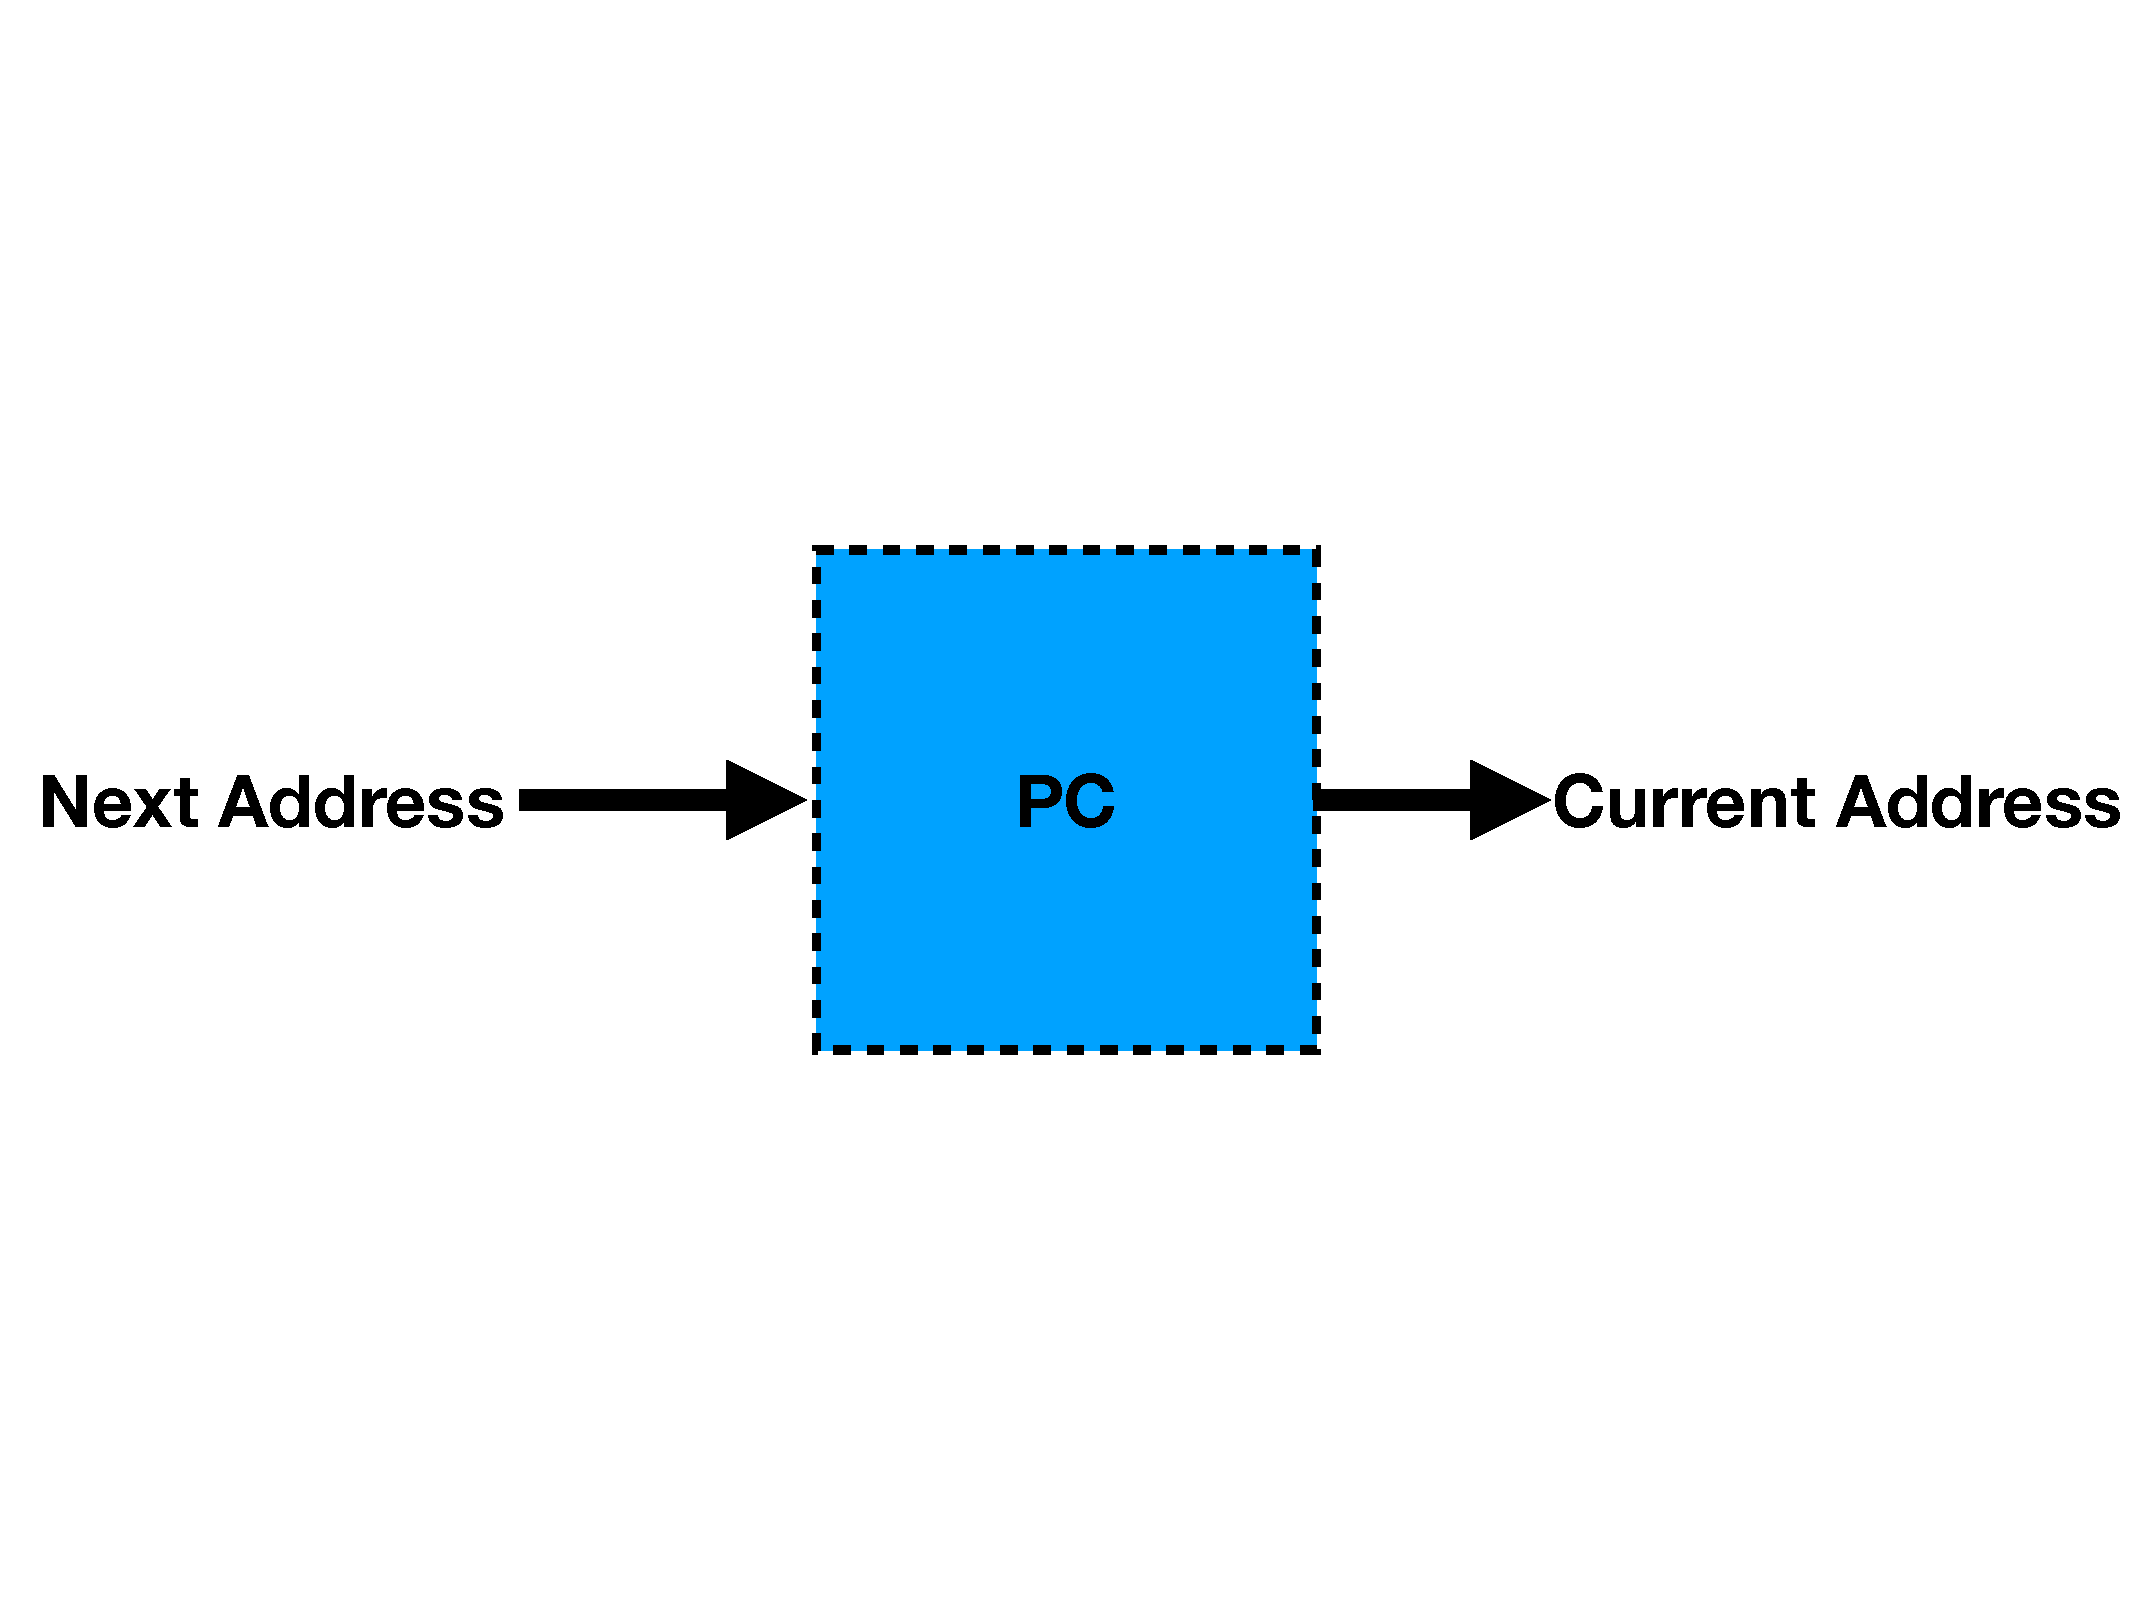
\includegraphics[scale=0.25]{pictures/PC.pdf}
            \caption{Illustration of the clocked \texttt{program counter} process having the next address as input and current address as output.}
            \label{fig:PC}
        \end{figure}
    
        \begin{minipage}{\linewidth}
            \begin{lstlisting}[language={[Sharp]C}, caption={A slice of the PC unit SME code, which contains variable that holds the input address. On every cycle edge it then holds and outputs the current address.},captionpos=b, label = PCSME]
...
    ulong address_hold;

    protected override void OnTick() {
        address_hold = m_Input.Address;
        Output.Address = address_hold;
    }
            \end{lstlisting}
        \end{minipage}   
    
    \subsection{Instruction Memory}
        The \textit{instruction memory}, IM for short, contains the program to be run on the CPU. To implement the instruction memory we create a SME process. It contains a byte array with the instructions to be run. A byte array was chosen to respect the conventions discussed in \ref{section:datatranserinstructions}. This also has the added benefit of having a built-in C$\scalerel*{\#}{X}$ function to read a binary file, which automatically puts the instructions contained within the file, in the correct array format. 
        
        The instructions can also be hand written when declaring the array. Since an instruction is 32-bits, 4 elements in the array are needed to form an instruction, where index 0-3 contains the first instruction.
        
        The instruction memory process has a single input from the program counter, which it uses access the correct instructions. In each cycle we first check whether the address given lies within the instruction array range, if not we shut down the CPU.
        We then construct an instruction, using methods discussed in \ref{section:Operators}, to a temporary variable.
        
        The register fields are then sliced out of this variable and put in the corresponding output buses, \texttt{Read RS1, RS2} and \texttt{Write RS}. The full instruction is also outputted to its own bus, \texttt{instruction}. Lastly we tell the simulation process to keep the CPU running by asserting the \texttt{CPU} bus. The instruction memory process has been illustrated in Figure \ref{fig:IM} and a code segment is shown Listing \ref{IMSME} explaining parts of the code. 
     
        \begin{figure}[h!]
            \centering
            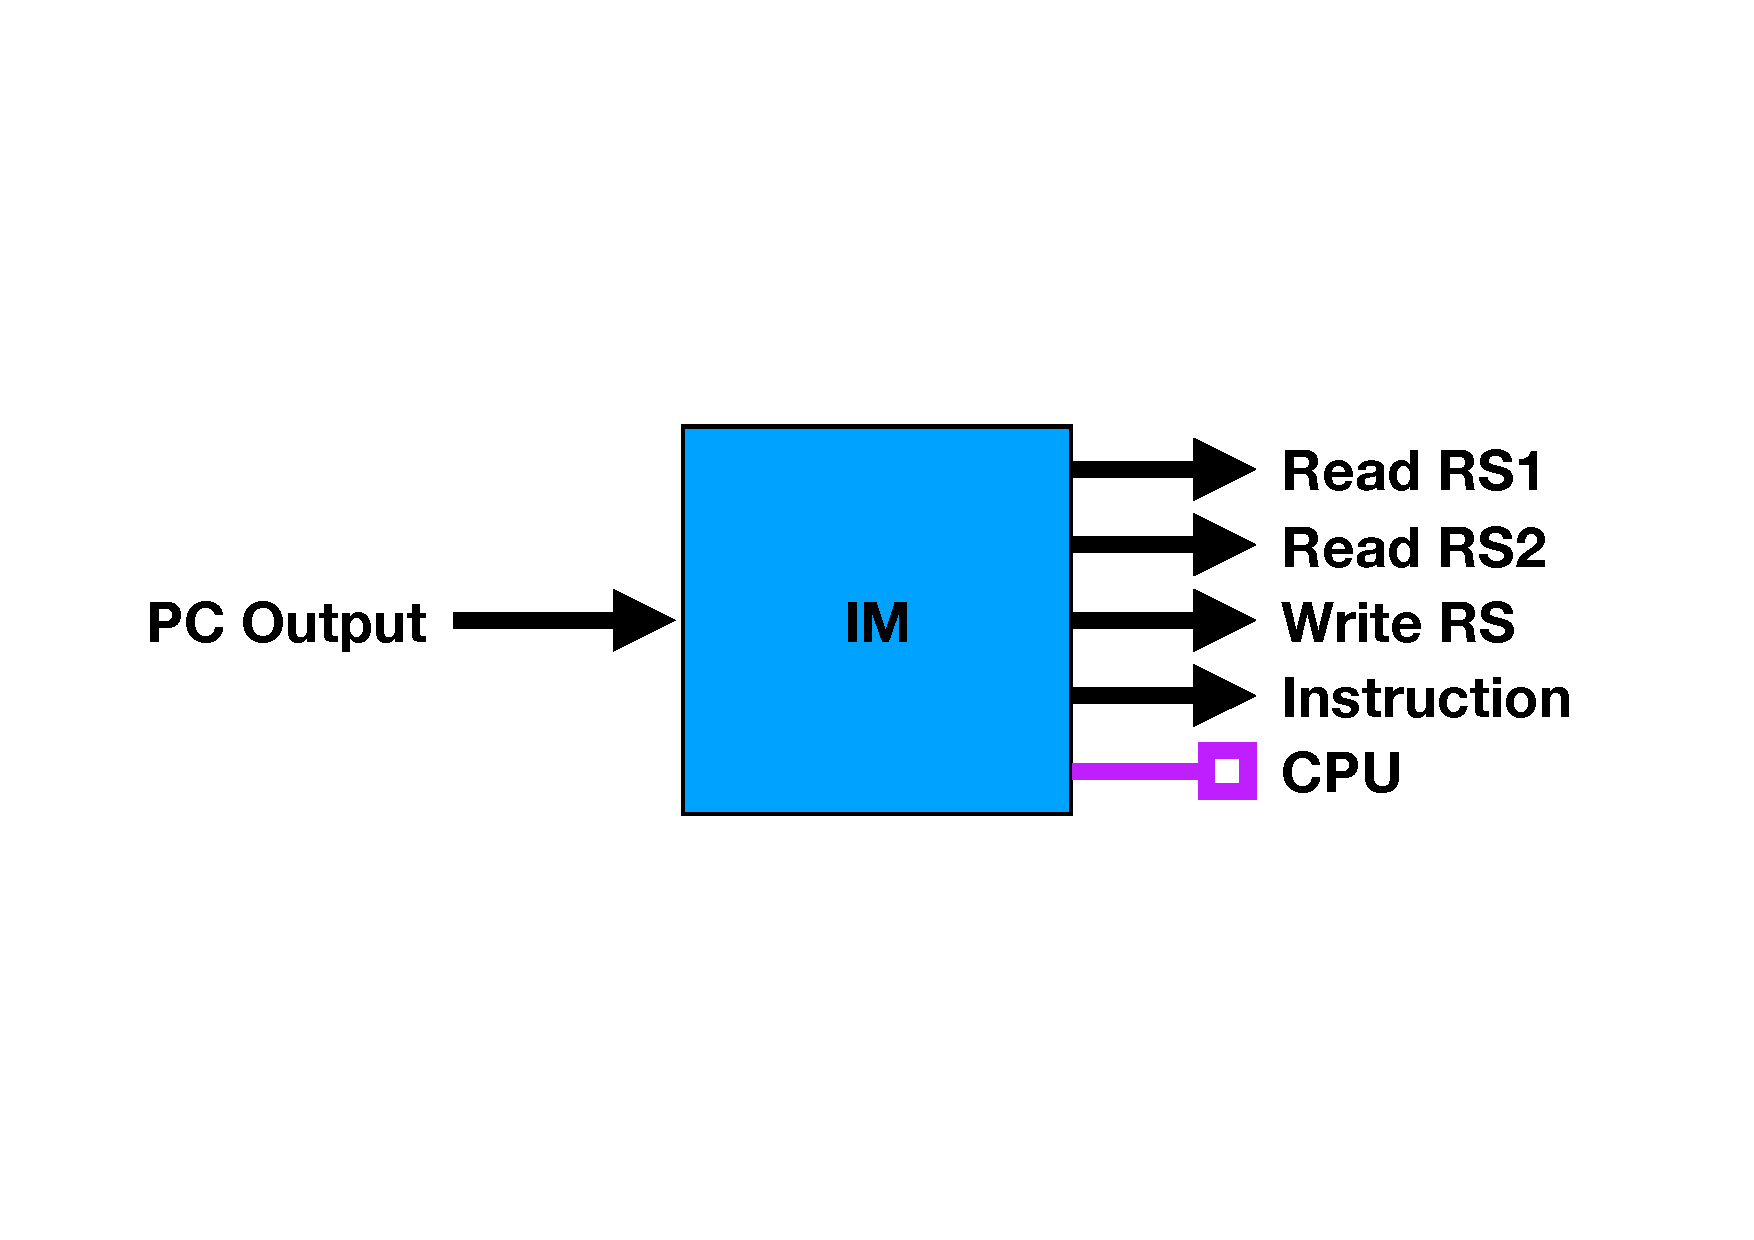
\includegraphics[scale=0.34]{pictures/IM.pdf}
            \caption{Illustration of the \texttt{instruction memory} process, taking the PC output as input and outputting to the 5 buses, \texttt{Read RS1 and RS2}, \texttt{Write RS}, \texttt{Instruction} and \texttt{CPU}.}
            \label{fig:IM}
        \end{figure}
    
        \begin{minipage}{\linewidth}
            \begin{lstlisting}[language={[Sharp]C}, caption={A slice of the Instruction Memory unit SME code. It contains a single byte array, which holds all the instructions to be run. First we check whether the given address to be accessed lies within instruction array, if not we shut down the CPU. We then use the address to access the correct array elements to create a temporary variable, which contains the instruction, as shown in lines 9-12. Hereafter we slice out the fields in the instruction and place the values in the correct busses. Lastly we tell the simulator to keep the CPU running using the CPU bus.},captionpos=b, label = IMSME]
...
    private readonly byte[] Instruction_Memory = System.IO.File.ReadAllBytes("/Users/danielramyar/Downloads/fibo.bin");
            
    protected override void OnTick() {
        ulong temp_address = m_input.Address;
        uint temp_instruction;
            
        if (temp_address >= 0 && temp_address < (uint)Instruction_Memory.Length) {
            temp_instruction = 0u | (uint)Instruction_Memory[temp_address]     << 24
                                  | (uint)Instruction_Memory[temp_address + 1] << 16
                                  | (uint)Instruction_Memory[temp_address + 2] << 8
                                  | (uint)Instruction_Memory[temp_address + 3];
            
            m_Instruction.Current = temp_instruction;
            m_read_1.Address = (uint)temp_instruction >> 15 & (uint)31; 
            m_read_2.Address = (uint)temp_instruction >> 20 & (uint)31; 
            m_write.Address  = (uint)temp_instruction >> 7  & (uint)31; 
            
            m_CPU.Running = true; // Keep CPU running
        }
        else {
            temp_instruction = 0u; // No Instruction
            ...  // Same as in the if statement
            m_CPU.Running = false; // Turn of cpu no more instructions
    }
            \end{lstlisting}
        \end{minipage}  
        
        
        
    
    \subsection{Next instruction Unit}
        To calculate the address of the next instruction in the queue I have created a unit called \texttt{Next}. This unit is very simple, as its only function is to increment the value found in the PC output bus by 4. We increment by 4, since each instruction is 32 bits long and since our instructions are contained in a byte array, we need to move 4 bytes every time we want to access the following instruction. For example if we are placed at index 0, we would have to go to index 4 to access the next instruction (index 0-3 contains instruction 1 and index 4-7 the next).
        
        The next instruction process has the the output from the program counter as input and sends the incremented address to the \texttt{Next Output} bus. The \texttt{Next} process is illustrated in \ref{fig:NEXT} and a code segment is shown in Listing \ref{NEXTSME}.
        
        \begin{figure}[h!]
            \centering
            \includegraphics[scale=0.34]{pictures/Next.pdf}
            \caption{Illustration of the \texttt{next} process, taking the \texttt{PC output} as input and outputs the next instruction adress to the \texttt{next output} bus.}
            \label{fig:NEXT}
        \end{figure}
    
        \begin{minipage}{\linewidth}
            \begin{lstlisting}[language={[Sharp]C}, caption={A slice of the \texttt{Next} process SME code. Here we declare a temporary varible, which contains the program counter output. We increment the temporary variable by four and place it in the output bus.},captionpos=b, label = NEXTSME]
...
    ulong temp;
    
    protected override void OnTick() {
        temp = m_Input.Address + 4;
        Output.Address = temp;
    }
            \end{lstlisting}
        \end{minipage}  
        
    
    \subsection{Register}
        The \texttt{register}, or RS for short, is a small data storage location for operands of instructions among others (see Table \ref{table:RISCVRegister}). It can be accessed by specifying a register address in an instruction. 
        
        Since R-type instructions use two operands to execute an arithmetic operation, the register has two input lines carrying the address to the specified registers and two output lines carrying the data in the read registers.
        
        Furthermore the result needs to get stored, therefore we need two additional lines one carrying the result of an operation and the other an address for the storage location. To avoid any unintentional write backs to the register, we introduce a write control line, which is asserted if write back is intended.
        
        In SME the register is declared as a process containing a signed 64-bit array with 32 entries. To ensure the latest data is always read, we write to the register as the first thing. Since register 0 is hard-wired to zero according to the conventions, we make sure that the write back address lies within the range 1-31 and that the write control is asserted.
        Lastly we check if the read addresses lies within the range of the register and then output the data in the read registers to the corresponding buses. The \texttt{register} process is illustrated in Figure \ref{fig:REGISTER} and a code segment shown in Listing \ref{REGISTER}.
    
        \begin{figure}[h!]
            \centering
            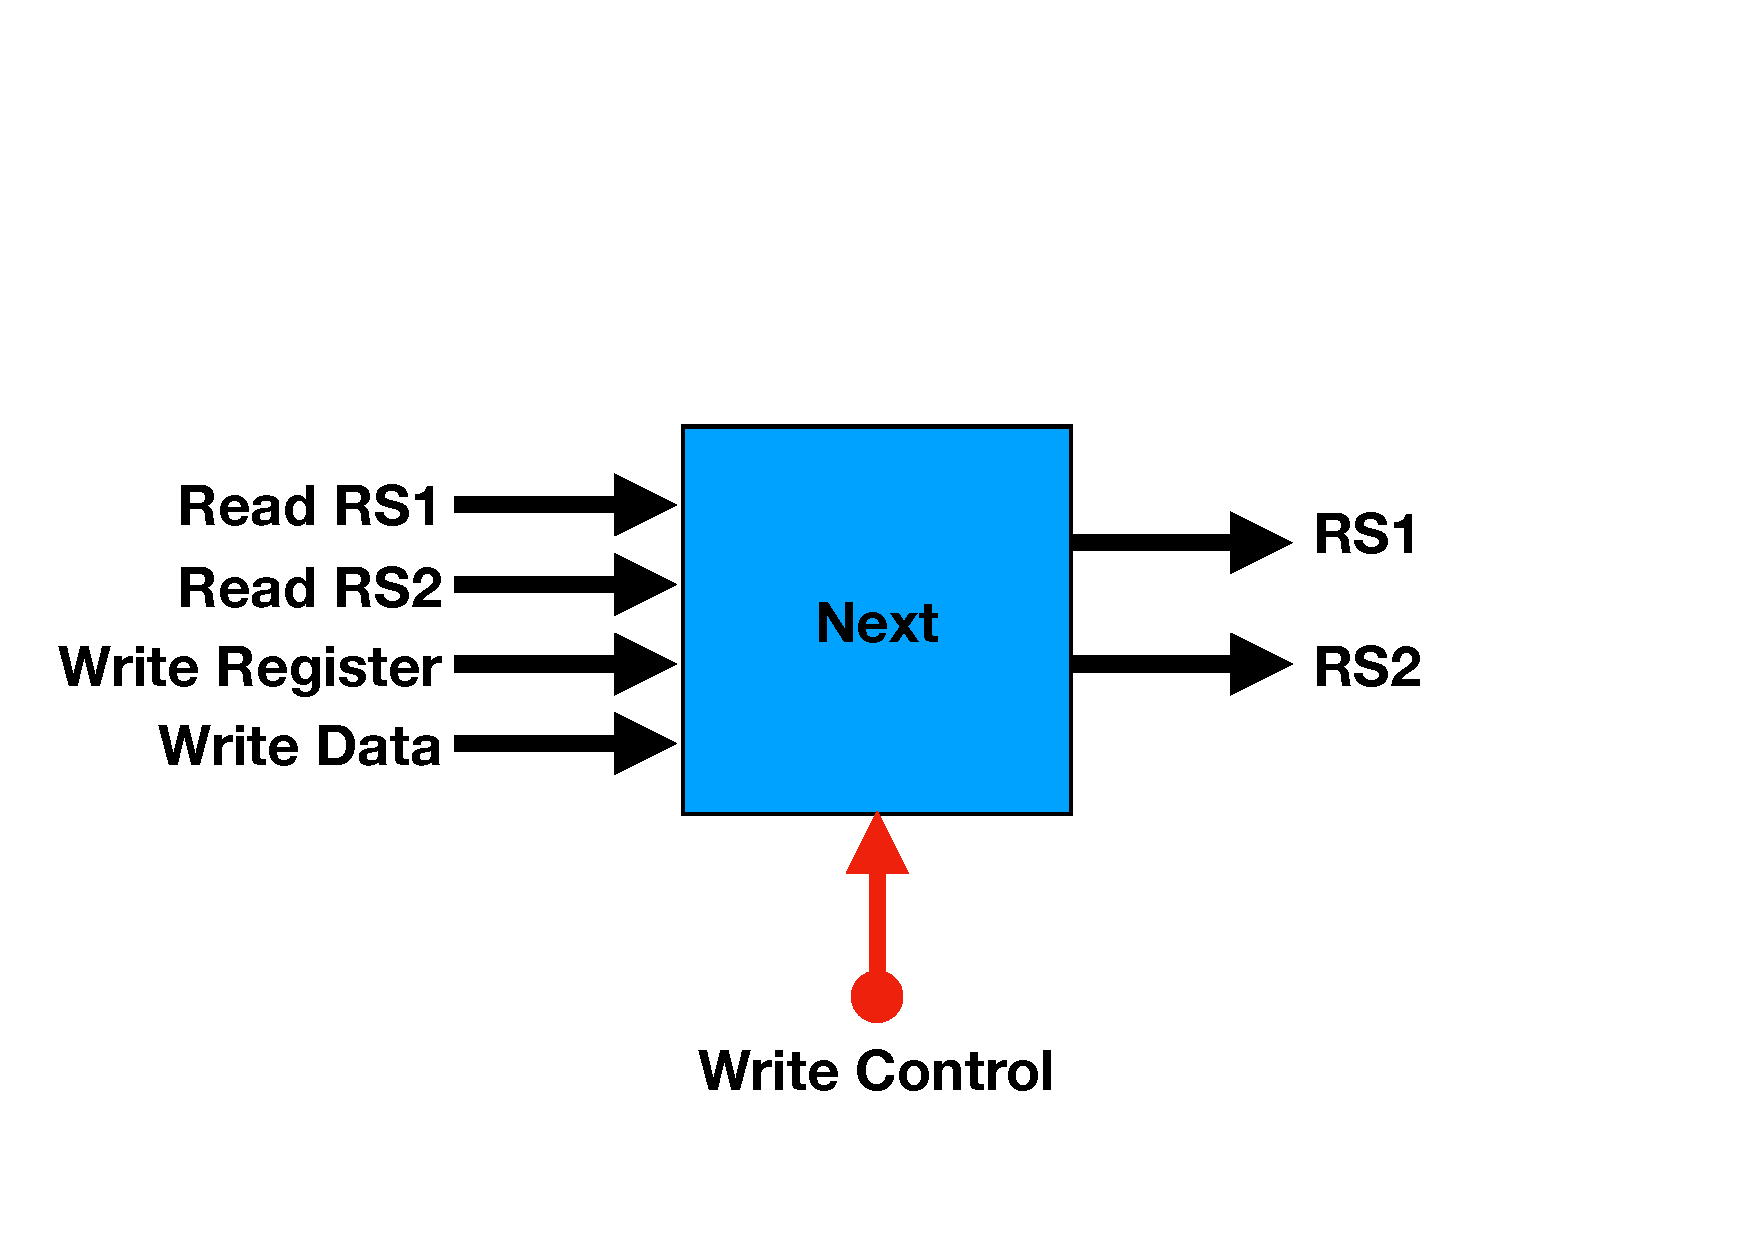
\includegraphics[scale=0.29]{pictures/REGISTER.pdf}
            \caption{Illustration of the \texttt{register} process. It gets its information on which register addresses to read from \texttt{Read RS1, RS2} buses. To write data the register uses \texttt{write register} bus to know which register to write to, the \texttt{write data} bus contains the data to be written and the \texttt{write control} bus authorize whether the register should write or not.}
            \label{fig:REGISTER}
        \end{figure}
    
        \begin{minipage}{\linewidth}
            \begin{lstlisting}[language={[Sharp]C}, caption={A slice of the \texttt{register} process SME code. The register is declared as a signed 64-bit array with 32 elements. In every clock cycle the process checks if the write control signal is asserted. If it is we check if the address to be written lies within the register range and is above 0, as this register is reserved to be hard-wired zero. Lastly the process reads the two specified registers and if they lie within the register range, they get outputted to the corresponding buses.},captionpos=b, label = REGISTER]
...
    private readonly long[] m_register = {0, 0, 0, 0, 0, 0, 0, 0,
                                          0, 0, 0, 0, 0, 0, 0, 0,
                                          0, 0, 0, 0, 0, 0, 0, 0,
                                          0, 0, 0, 0, 0, 0, 0, 0,};
            
    protected override void OnTick() {
        if (m_write_control.Enable == true && m_write.Address > 0 && m_write.Address < 32) {
            m_register[m_write.Address] = m_write_data.Data;          
        }
        if (m_read_1.Address >= 0 && m_read_1.Address < 32) { 
            output_1.Data = m_register[m_read_1.Address];
        }
        if (m_read_2.Address >= 0 && m_read_2.Address < 32) { 
            output_2.Data = m_register[m_read_2.Address];
        }
    }
            \end{lstlisting}
        \end{minipage}  
    
    \subsection{Arithmetic Logic Unit (ALU)}
        The \texttt{Arithmetic Logic Unit}, or ALU for short, is the computational powerhouse of the CPU. It is here all arithmetic, logical, shift and bitwise operations are computed.
        The ALU has two inputs that consists of the operands of an operation. The output is then the result. To determine which operation to perform we additionally have a control line with the operation code or opcode.
        
        In the SME implementation all the operations are enclosed in a \texttt{switch} statement, that is controlled by the opcode to determine which operation to execute. The ALU is illustrated in Figure \ref{fig:ALU} and a code segment is shown in Listing \ref{ALU}.
    
        \begin{figure}[h!]
            \centering
            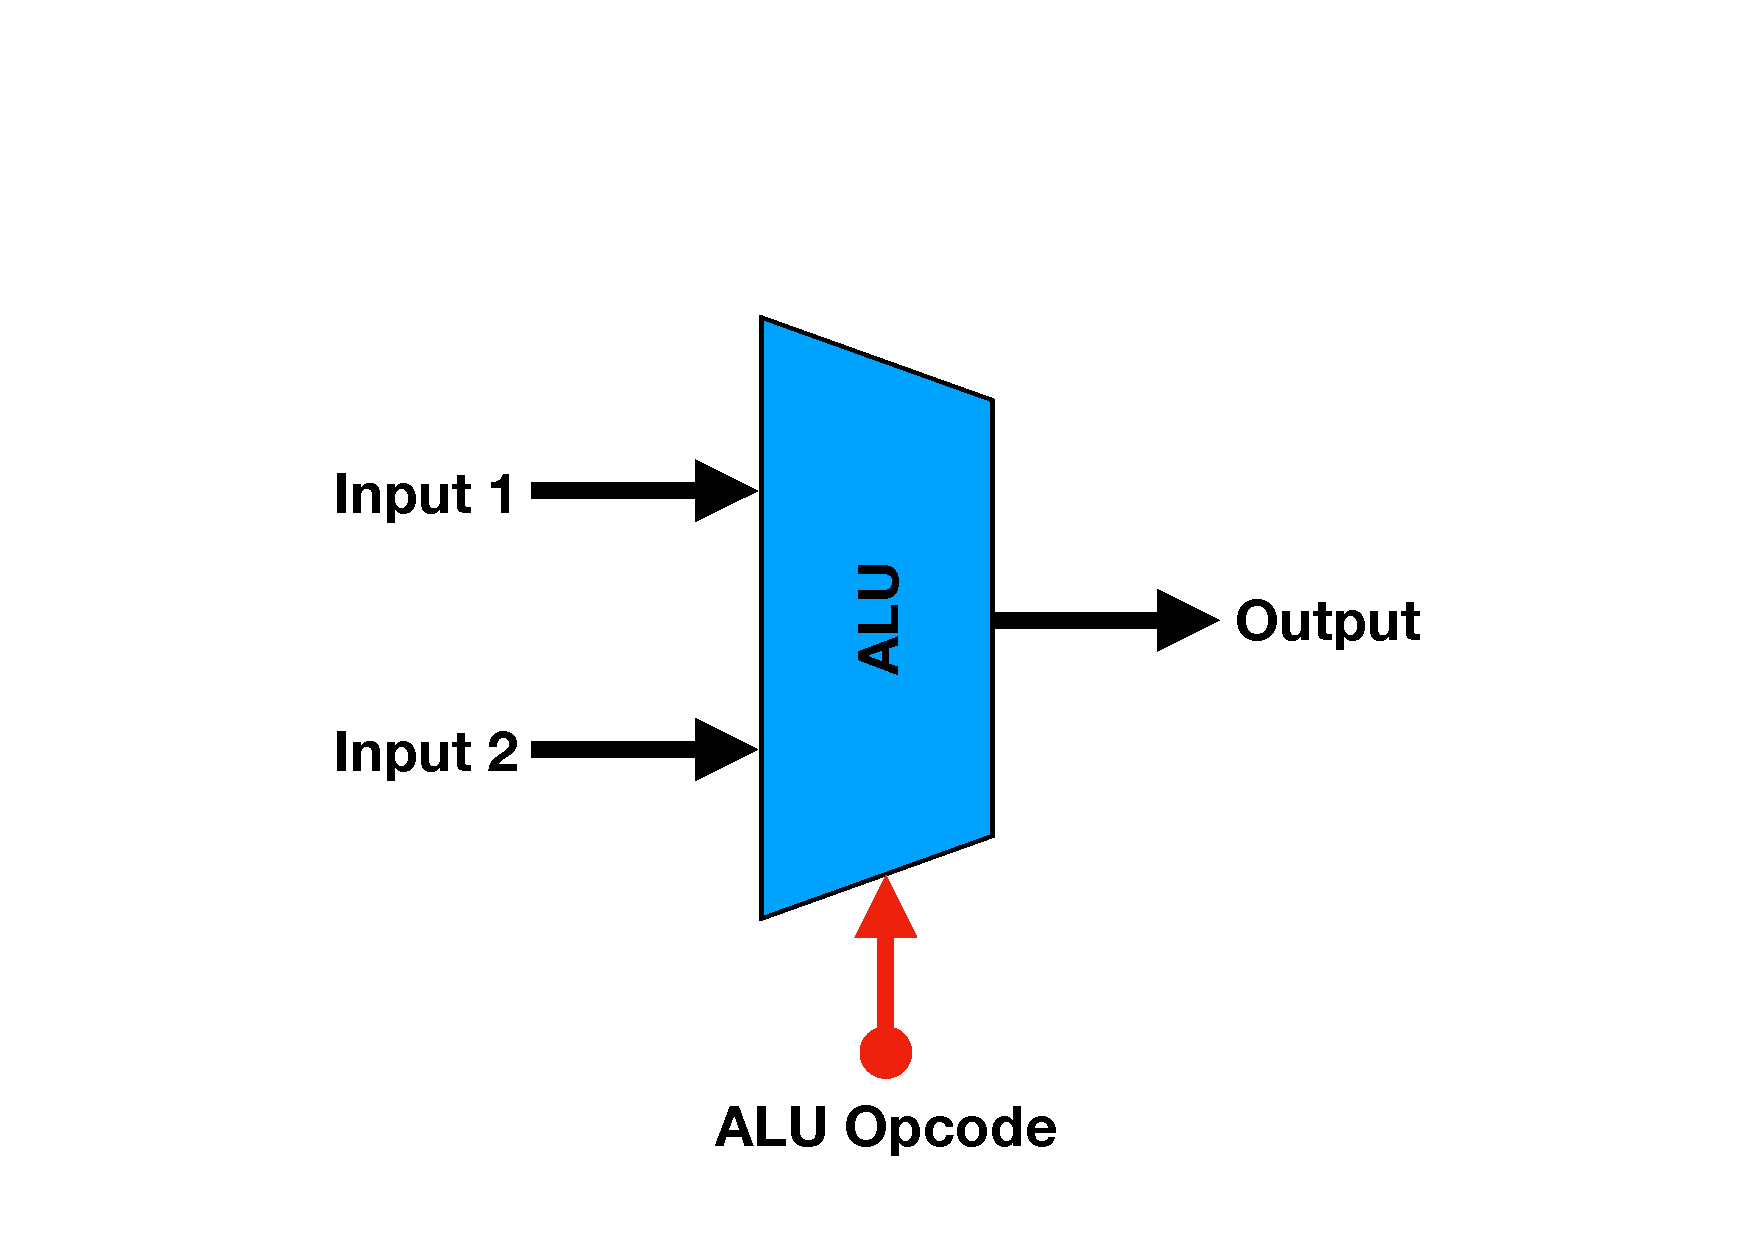
\includegraphics[scale=0.32]{pictures/ALU.pdf}
            \caption{Illustration of the \texttt{ALU} process. The two input contains the operands of the operation to be executed and the output is the result. The ALU opcode (in red) controls which operations the ALU will perform.}
            \label{fig:ALU}
        \end{figure}
    
        \begin{minipage}{\linewidth}
            \begin{lstlisting}[language={[Sharp]C}, caption={A slice of the \texttt{ALU} process SME code. The ALU consists of a large \texttt{switch} statement, with cases for each operation to be performed, which is controlled by the ALU operation code (\texttt{opcode}). },captionpos=b, label = ALU]
...
    protected override void OnTick() {
        switch (m_ALUOP.Value) {
            case 0:
                output.Value = m_ALU_In_1.Data + m_ALU_In_2.Data;   // ADD
                break;
            case 1:
                output.Value = m_ALU_In_1.Data - m_ALU_In_2.Data;   // SUB
                break;
            case 2:
                output.Value = m_ALU_In_1.Data & m_ALU_In_2.Data;   // AND
                break;
            case 3:
                output.Value = m_ALU_In_1.Data | m_ALU_In_2.Data;   // OR
                break;
            case 4:
                ...
        }
    }
            \end{lstlisting}
        \end{minipage}  
        
    
    \subsection{Immediate generator}
        The \texttt{Immediate Generator}, or IMMGEN for short, extracts immediate fields from instructions. This is a pretty large unit since it needs to know where the immediate field is located in every instruction. To make matters worse some immediate fields in the instructions are totally scrambled, so we have to be really careful on how we reconstruct them.
        
        To start we need to be able to identify which type of instruction we are dealing with to know where the immediate field is located. Luckily almost all types of instructions have a unique operation code (for example the I-type has opcode 19), we therefore use a \texttt{switch} statement in the SME code with the opcode in the instruction as a branching condition to identify the instruction type.
        
        Some instructions of same type, only use the lower 6 bits in the immediate field, such as the \texttt{slli} instruction. To accommodate this fact we make use of another \texttt{switch} statement, within the specific case of the first \texttt{switch} statement, that uses the \texttt{funct3} field as branching condition, since this is the unique identifier within the same type of instruction (for example \texttt{opcode} 19, \texttt{funct3} 1 is the \texttt{slli} instruction).
        
        When we know where the immediate field is located it is time to extract it. This is done by shifting the instruction in question to the right, such that the first bit of the immediate field is located at bit index 0 of the 32-bit instruction. Hereafter we do a bitwise AND operation to remove all but the necessary bits (see Section \ref{section:Operators}). It should be noted that in cases, where the immediate field only is 12-bits long we need to perform a shift to the left and then right to retain the sign bit, as 12-bit numbers are not supported by \texttt{C\#} and therefore does not happen automatically, when cast to \texttt{long} type.
        
        If we deal with \texttt{B-} and \texttt{J-type} instructions, we need to be really careful when we reconstruct the immediate field, as the immediate field bits do not lie in a trivial manner. An important thing to note is that in these types of instructions the first bit is not supplied and therefore should not get shifted all the way to the 0'th bit index but should get shifted to the 1'st bit index. This firstly ensures that we only jump by an even number of bytes, as this is where the base index is for the instructions and we effectively double the range we can jump instructions.
        
        When the immediate field is constructed it simply gets outputted as a signed 64-bit number. The immediate generator is illustrated in Figure \ref{fig:IMMGEN} and a code segment is shown in Listing \ref{IMMGEN}.
        
        
        \begin{figure}[h!]
            \centering
            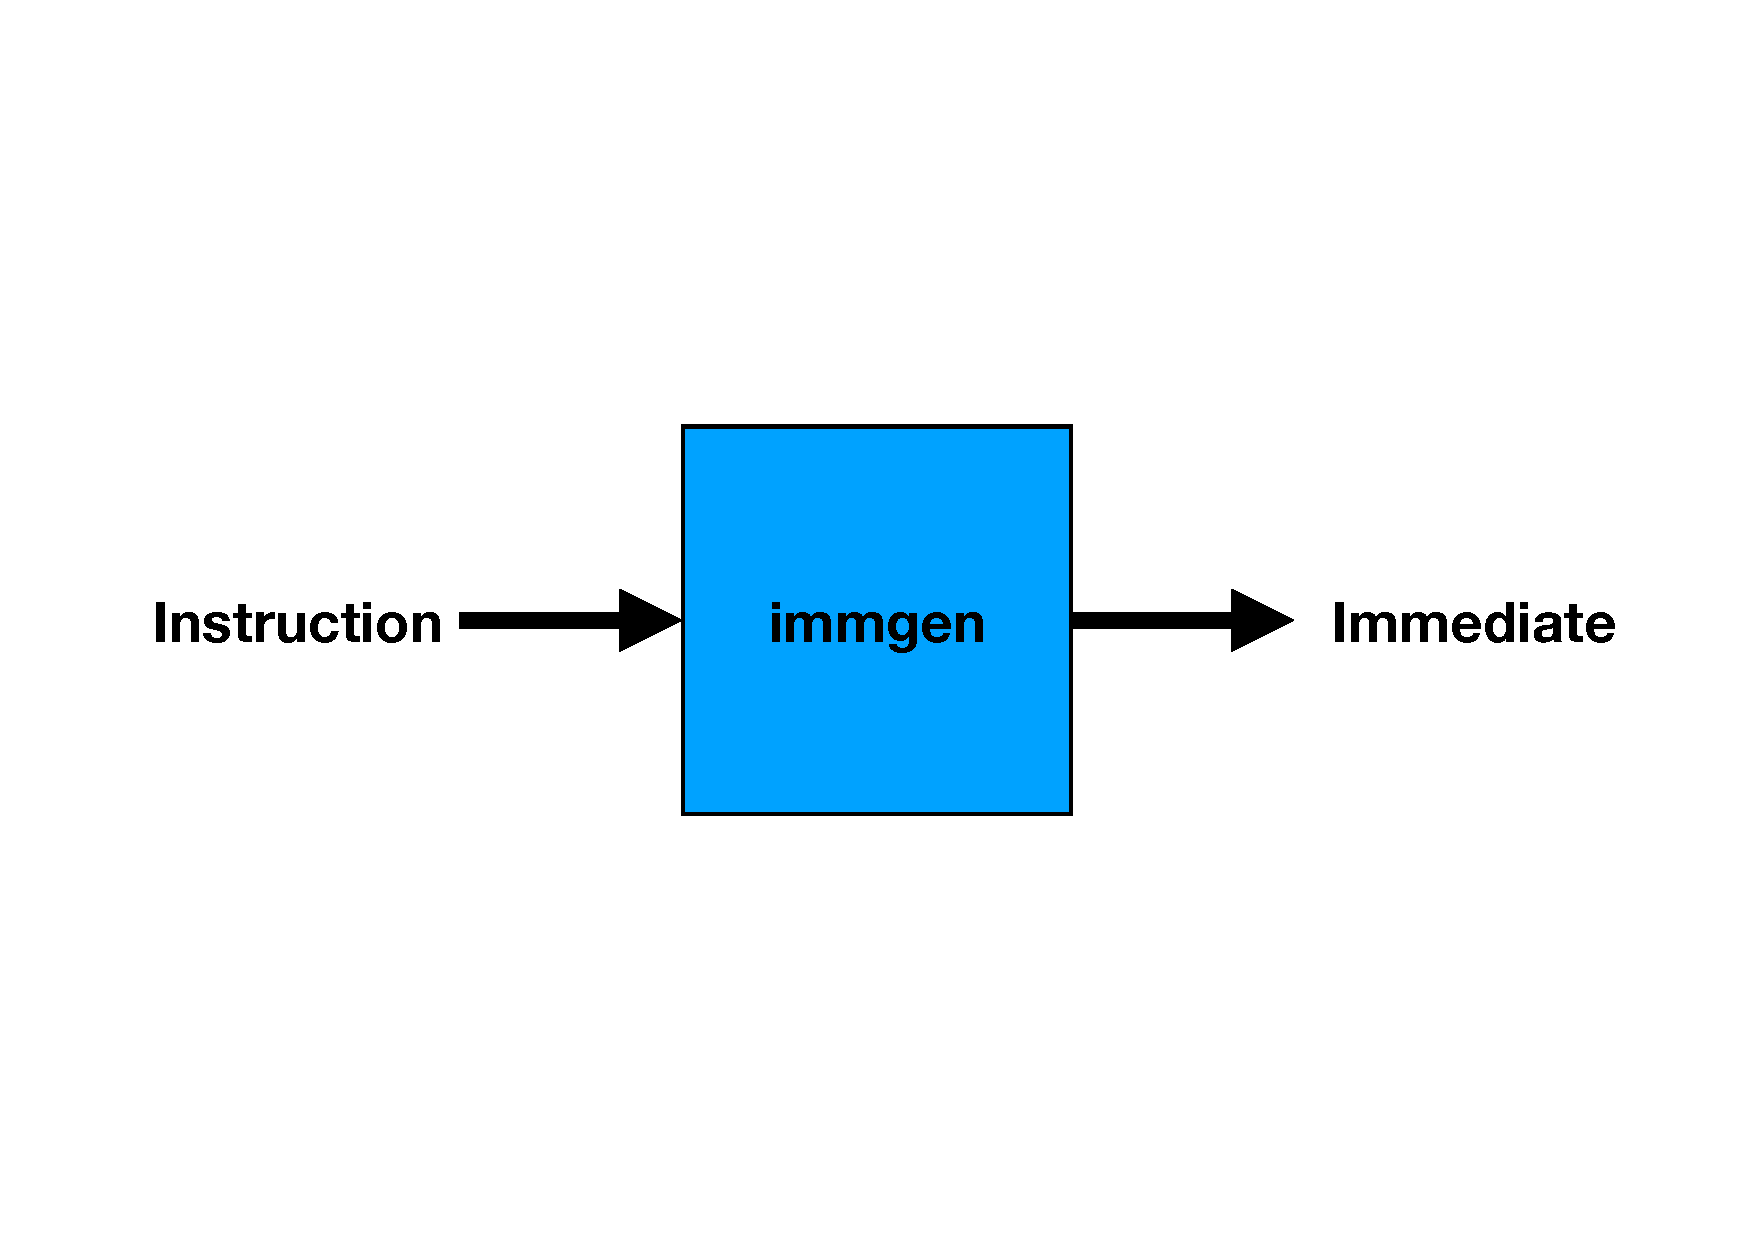
\includegraphics[scale=0.35]{pictures/IMMGEN.pdf}
            \caption{Illustration of the \texttt{immediate generation} process, taking an instruction as input. It then extracts the immediate field, which it outputs. }
            \label{fig:IMMGEN}
        \end{figure}
    
        \begin{minipage}{\linewidth}
            \begin{lstlisting}[language={[Sharp]C}, caption={A slice of the \texttt{IMMGEN} process SME code. We first extract the opcode and funct3 fields from the instruction and put them in a variable. We then use a \texttt{switch} statement and the opcode to determine what type of instruction we are dealing with. Since some instructions of same type like \texttt{slli} only use the lower 6 bits in the immediate field (shamt field), we need another switch statement to tell these apart using the funct3 field. Lastly we construct the immediate and output it . Note that in line 18 we make use of a little hack to retain the sign bit of a 12 bit number since it is not supported in \texttt{C\#}},captionpos=b, label = IMMGEN]
...
    protected override void OnTick() {
        uint Opcode = m_instruction.Current & (uint)0x7F;
        uint funct3 = m_instruction.Current >> 12 & (uint)0x7;
            
        switch(Opcode) {
            ...
            case 19:                                        // I-format
                switch (funct3) {
                    ...
                    case 5:
                        temp1 = m_instruction.Current >> 20 & (uint)0x3F;
                        temp0 = (long)temp1;
                        output.Immediate = temp0;
                        break;
                    default:
                        temp1 = m_instruction.Current >> 20 & (uint)0xFFF;
                        short temp5 = (short)((short)(temp1 << 4) >> 4);
                        temp0 = (long)temp5;
                        output.Immediate = temp0;
                        break;
                }
            break;
            case 27:                                        // I-format Word
                ....
        }
    }
            \end{lstlisting}
        \end{minipage} 
\newpage
    \subsection{Data Memory}
        The \texttt{Data Memory}, or DM for short, is the main data storage unit of the CPU, as it can contain much more data than the register.
        
        \begin{figure}[h!]
            \centering
            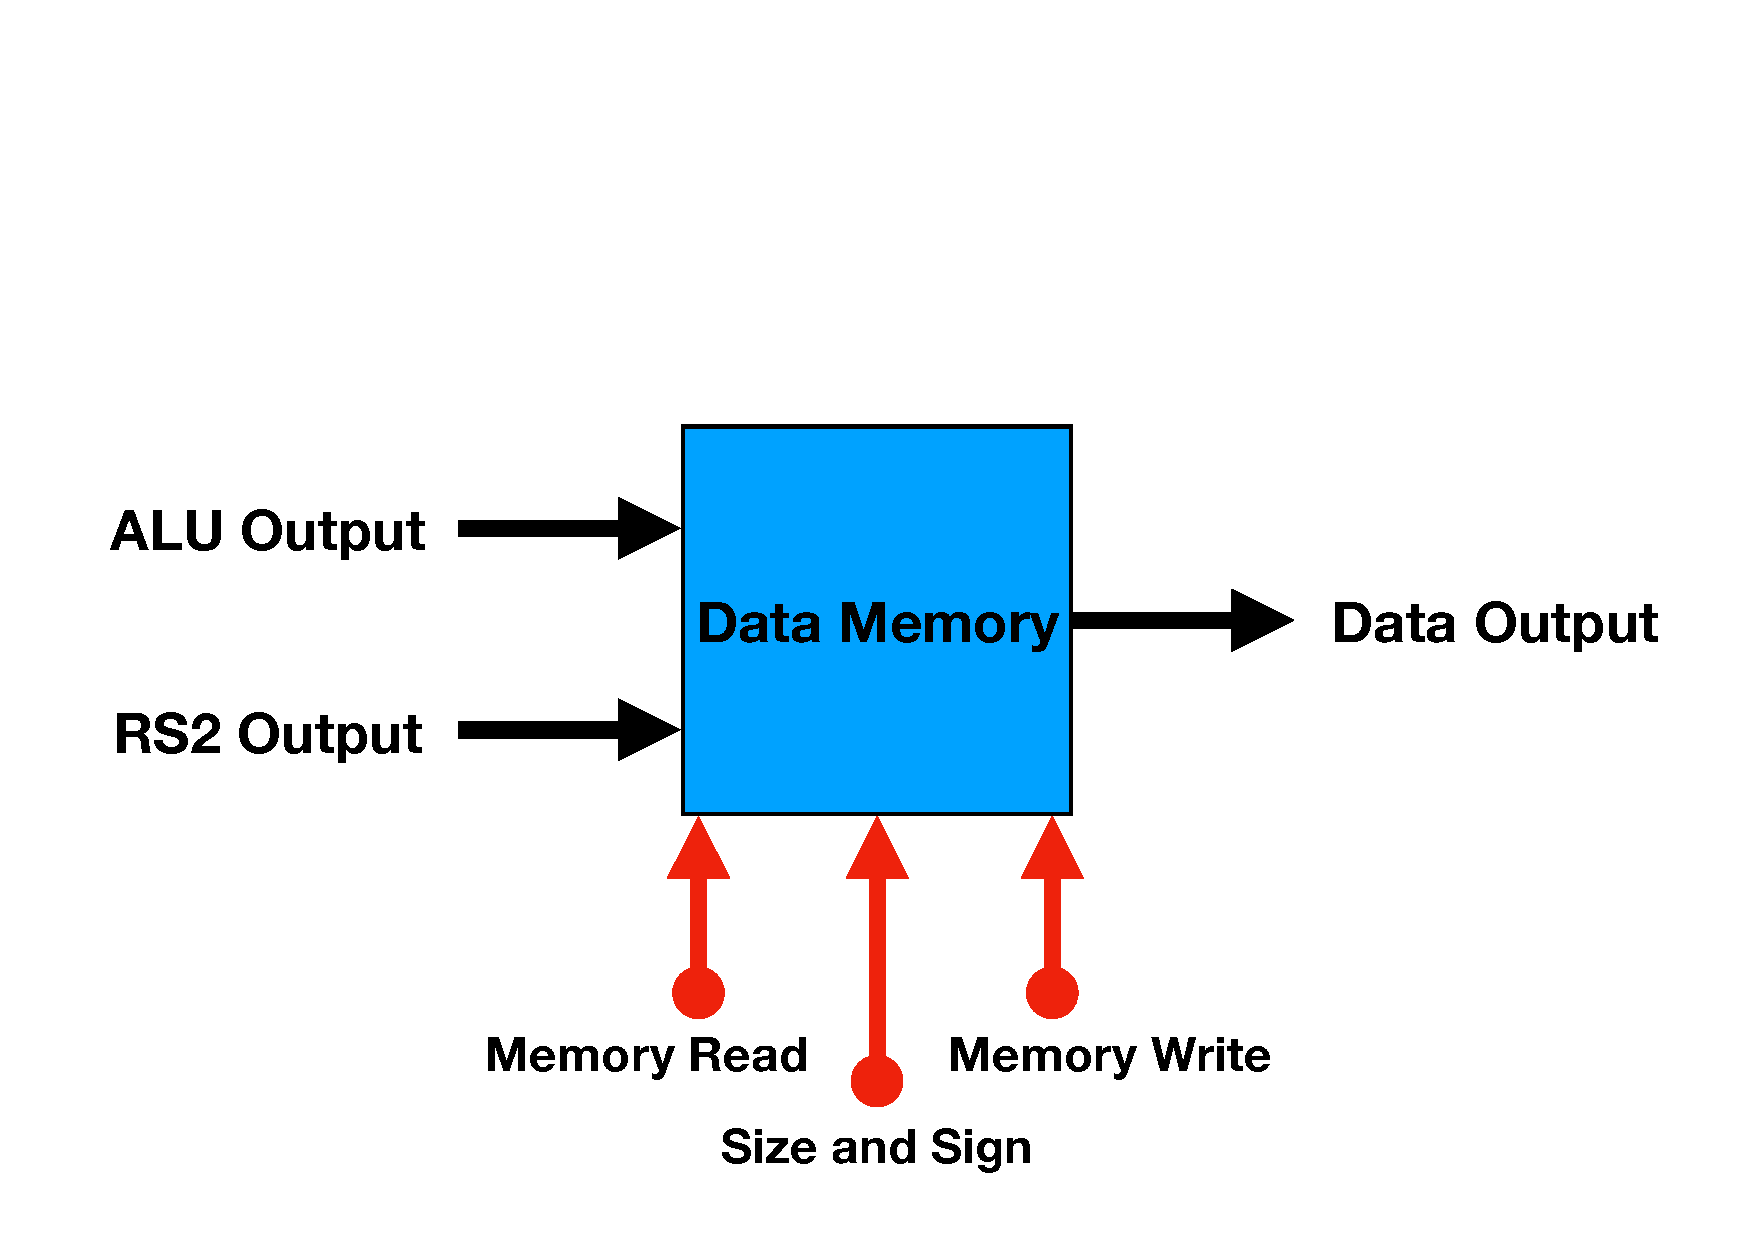
\includegraphics[scale=0.35]{pictures/DM.pdf}
            \caption{Illustration of the \texttt{Data Memory} process. As input it takes the result from the ALU and controls signals (in red) \texttt{Memory Read}, \texttt{Memory Write} and \texttt{Size and Sign}. It then outputs the read data or 0 if both \texttt{Memory Read} and \texttt{Memory Write} are deasserted.}
            \label{fig:DM}
        \end{figure}
    
        \begin{minipage}{\linewidth}
            \begin{lstlisting}[language={[Sharp]C}, caption={A slice of the \texttt{Data Memory} process SME code. Similar to the instruction memory, the data memory consists of a byte array, which we made 2000 elements long in this case. As there can only be read or written to the data memory once per clock cycle, we simply construct an \texttt{if/else} statement, which uses control signals to determine the procedure to be done. Both the read and write procedures needs to know the size and sign of the data to be loaded or written. Therefore a \texttt{switch} statement has been added to both outcomes, which uses \texttt{SizeAndSign} control signal to choose between the cases. When reading the data from memory we need to remember that it is little-endian addressed  so before we output the value the bits need to be shuffled around in the correct order, so the correct value is added to the register, as that is big-endian. When writing the data the opposite need to happen, so a big-endian value need to be converted to a little-endian one. If both read and write control signals are deasserted I choose to output 0.},captionpos=b, label = DM]
...
    byte[] Data_Memory = new byte[2000];
            
    protected override void OnTick() {
        if (m_MemRead.Enable) {
            ...
            switch (m_SizeAndSign.Value) {
                ...
                case 1: // load word
                    temp0 =
                    Data_Memory[m_Address.Value] | Data_Memory[m_Address.Value + 1] << 8
                                                 | Data_Memory[m_Address.Value + 2] << 16
                                          | (sbyte)Data_Memory[m_Address.Value + 3] << 24;
                    break;
                case 2: // load short
                    ...
            }
            output.Data = temp0;
        }
        else if (m_MemWrite.Enable) {
            switch (m_SizeAndSign.Value) {
                ...
                case 2:
                    Data_Memory[m_Address.Value]     = (byte)(m_Data_input.Data      & 0xFF);
                    Data_Memory[m_Address.Value + 1] = (byte)(m_Data_input.Data >> 8 & 0xFF);
                    break;
                case 3:
                    Data_Memory[m_Address.Value] = (byte)(m_Data_input.Data & 0xFF); 
                    break;
            }
        }
        else {
            output.Data = 0;
        }
    }
            \end{lstlisting}
        \end{minipage} 
    
\section{Designing the Control}
    
\section{Single Cycle RISC-V datapath}

\section{Improving the datapath} \improvement{figure out better naming for sections}

    \subsection{RV64I Base Instructions Support}

    \subsection{Supporting R-Format}
    
    \subsection{Supporting I-Format}
    
    \subsection{Supporting S-Format}
    
    \subsection{Supporting B-Format}
    
    \subsection{Supporting U-Format}
    
    \subsection{Supporting J-Format}
    
\section{Debugging the instructions}

    \subsection{Writing assembly to test instructions}
    
    \subsection{Writing simple C code to run on RISC-V}
    
    
    

    